% \section{Introduction}
% Geographic information system (GIS) data are openly available for a variety of applications. Data~on terrain height and type have historically been available, with high-accuracy labeled data now increasingly available, e.g., building footprints and heights.  Systematic characterization of building roof architecture and slope offers a new dimension to traditional terrain data.  These data could be used to rapidly identify building change or damage from the air, to improve in-flight localization capabilities in GPS-denied areas, and to inform small Unmanned Aircraft Systems (UAS) of alternative ditching sites, a problem previously investigated by the authors \cite{ochoa_fail-safe_2017, castagno_comprehensive_2018}.   Databases such as OpenStreetMap (OSM)~\cite{openstreetmap_contributors_planet_2017} provide limited roof information, but such data have been manually entered to-date thus is~sparse. 


This chapter summary describes research to fuse satellite imagery and airborne Light Detection and Ranging (LiDAR) data through multiple stages of machine learning classifiers to accurately characterize building rooftop shape.  With these results, roof geometries worldwide can be stored in an easily-accessible format for UAS, GIS, or other applications. Supervised training datasets are generated by combining building outlines, satellite, and LiDAR data. The resulting annotated dataset provides individual satellite image and LiDAR (depth) image representations for each building roof. Roof shapes are automatically categorized through a combination of convolutional neural networks (CNNs) and classical machine learning. Transfer learning is employed in which multiple pre-trained CNN model architectures and hyper-parameters are fine-tuned and tested. The best-performing CNN for both satellite and LiDAR data inputs is used to extract a reduced feature set which is then fed into either support vector machine (SVM) or random forest classifiers to provide a single roof geometry decision.  Validation and test set accuracies are evaluated over a suite of different classifier options to determine the best model(s). A range of urban environments are used to train and test the proposed models. Data from Witten, Germany; Ann Arbor, Michigan; and the Manhattan borough of New York City, New York are collected and manually labeled to represent small to large metropolitan city centers. We show that combining datasets from both small and large cities leads to a more generalized model and improves performance. Figure \ref{fig:outline_methods} provides an overview of the data processing pipeline and illustrates a {UAS localization and contingency landing} use case. %\cite{Castagno2018ICUAS}.

\begin{figure}[ht]
\centering
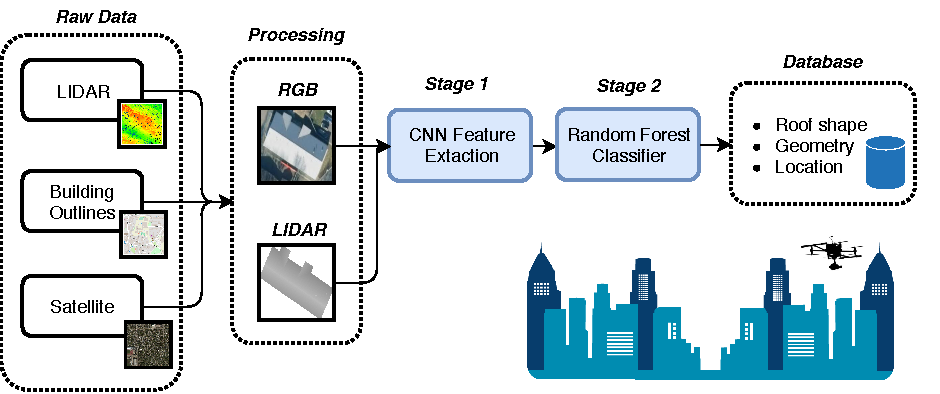
\includegraphics[width=0.70\textwidth]{chapter_4_roofshape/imgs/overview_process.pdf}
\caption{Roof classification data fusion and processing pipeline. LiDAR, building outlines, and satellite images are processed to construct RGB and LiDAR images of a building rooftop. In Stage    1, these images are fed into a CNN for feature extraction, while Stage    2 uses these features with a random forest for roof classification. These data can be stored for quick reference, e.g., navigation or emergency landing site~purposes. }
\label{fig:outline_methods}
\end{figure}




\paragraph{Results}

After training and validating a multitude of machine learning architectures, the best model is selected to be evaluated on two independent test sets. Test Set 1 comes from the 20\% withheld data representing the cities of Witten and New York City. The second test set from Ann Arbor is completely independent; the model was never trained on data from this region. The total accuracy for Test Set 1 is 87.2\%, while Test Set 2  scored 86.7\%. Confusion matrices for both test sets are shown in Figure  \ref{fig:ch1_dual_tes_cm}. The row-wise percentage of each cell is computed and color-coded along with the specific quantity classified in parentheses underneath. For both test sets one of the largest error sources is confusion between \texttt{complex-flat} and \texttt{flat} roofs.
For urgent landing use cases, both classes may be combined to a final ``flat-like'' class. To ensure only reliable predictions one can apply a confidence threshold for prediction. An 80\% confidence threshold results in a precision of 95\% with a recall of greater than 70\%. 


% The~authors found difficulty in labeling some flat-like roof examples, especially ones that bear traits of both classes; it is clear this confusion carried over into the trained model. In some cases, a roof is on the threshold of being \texttt{flat} or \texttt{complex-flat}, and this ambiguity makes it difficult to provide a consistent ``correct'' answer.  Indeed, this case often applies between the \texttt{complex-flat} and \texttt{unknown} labels as well:  When~does a~\texttt{complex-flat} roof become too complex to support a safe small UAS landing? The~authors attempted to be consistent in answering this question when labeling data, however edge cases were observed. 

% Table \ref{table:quality_metrics1} and \ref{table:quality_metrics2}  list  results for recall (completeness), precision (correctness), and~quality for Test Set     1 and Test Set     2, respectively. Note that there were no \texttt{pyramidal} roofs shapes in the Ann Arbor test set and too few \texttt{half-hipped} and \texttt{skillion} roofs to calculate valid metric~results.


\begin{figure}[ht]
    \centering
    \begin{subfigure}[t]{0.45\columnwidth}
        \centering
        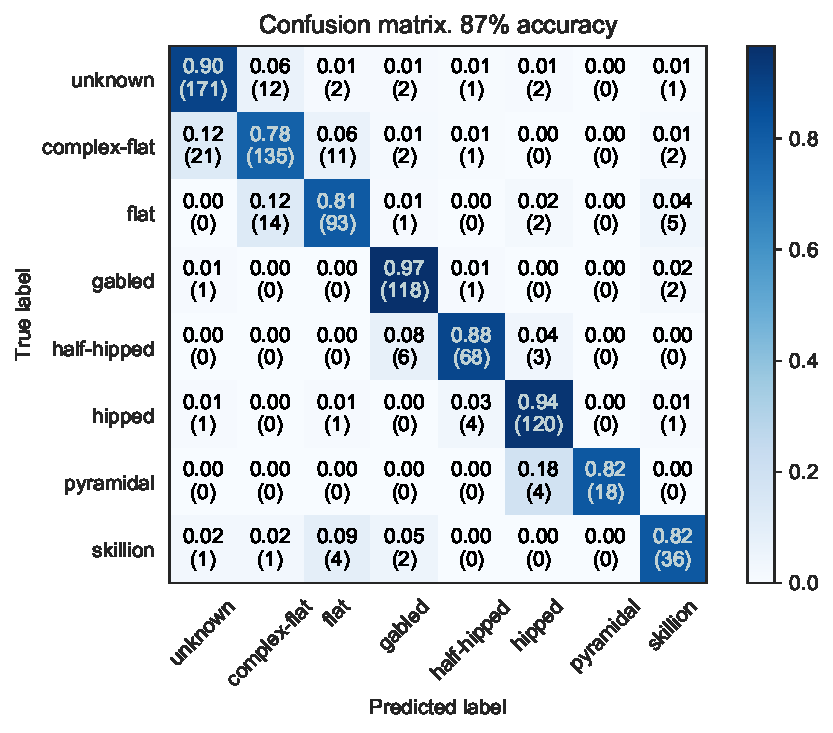
\includegraphics[width=0.90\textwidth]{chapter_4_roofshape/imgs/allclasses_combined_dual.pdf}
        \caption{Test Set     1}
        \label{fig:ch1_dual_test_combined_cm}
    \end{subfigure}
    \hfill
    \begin{subfigure}[t]{0.45\columnwidth}
        \centering
        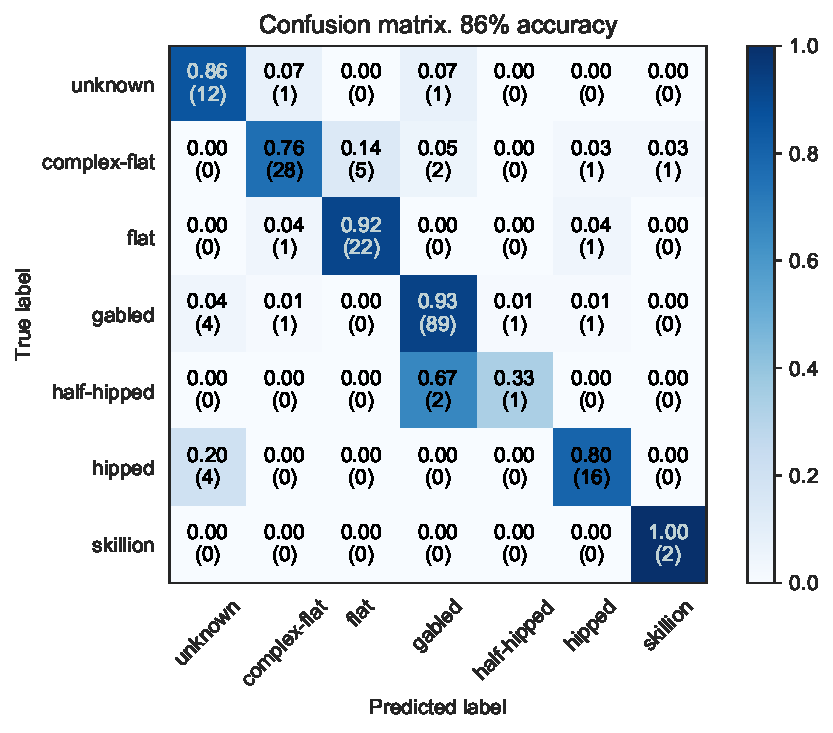
\includegraphics[width=0.90\textwidth]{chapter_4_roofshape/imgs/allclasses_aa_annarbor_dual.pdf}
        \caption{Test Set     2}
        \label{fig:ch1_dual_test_annarbor_cm}
    \end{subfigure}
    \vspace{-1pt}
    \caption{Confusion Matrices for Test Set 1 (Witten/Manhattan) and Test set 2 (Ann Arbor). }
    \label{fig:ch1_dual_tes_cm}
    \hfill
\end{figure}

\vspace{-1cm}
\paragraph{Conclusion}
Satellite images, LiDAR point clouds, and building outlines were processed to construct individual image representations of depth and color of roof shapes.  The final model uses deep learning for feature extraction and a random forest algorithm for subsequent roof shape classification. Generalized models and test datasets show promise for applying machine learning to automatically label roof shapes around the world with high confidence.
Full analysis of all models and results can be found in our paper \cite{castagno_roof_2018}.


% \begin{itemize}
%     \item Over 4500 building roofs spanning three cities have been manually classified and archived with a satellite and LiDAR depth image pair. This dataset is released with this paper.%NOTE: ?4500?
%     \item A ``complex-flat'' and ``unknown'' roof shape classe enable the machine classifier to distinguish flat roofs with infrastructure (e.g., air conditioning and water towers), unfamiliar roof shapes, and~images of poor quality.
%     % \item This paper significantly reduces the set of outliers that previously required manual removal for training and test datasets (from 45\% in \cite{Castagno2018} down to 5\% in this paper). This paper's test set accuracies represent a reasonable expectation of results when deployed in new areas.
%     \item An analysis of confidence thresholding is presented to improve the model's predictive power. This ensures only correct labels are assigned which is critical for use in high risk scenarios. 
%     \item Expanded results are presented from use of a single trained classifier (over Witten and Manhattan) tested with datasets from three cities, one of which (Ann Arbor) was never used for training or~validation.
% \end{itemize}

% The paper is structured as follows.  First, GIS data sources and prior roof geometry classification work are summarized.  Next, background in machine learning and data extraction methods is provided.  Specific methods to extract data for input to this paper's machine learning feature extraction and classification system are presented, followed by a description of training, validation, and test runs performed.  Statistical accuracy results are presented followed by a discussion and conclusions.